\section{Networks in molecular biology}

% Make the case for pathways and gene interactions - Why it is important to study them
Interactions and the relationship between multiple components are an important component of the biological functioning. There are multiple levels of interactions in the molecular biology which are represented by gene pathways, where one gene influences another to produce more or less of a protein, and that in turn produces more proteins and so on until that pathway fulfil its function. When something goes wrong in the body as in the case of the cancer, a certain pathways is altered and it is not working as intended. Thus, it is of great importance to understand, model and analyse these interactions.

% Introduce graph and network theory
Network or graph theory is the branch of the mathematics that models the interactions between multiple elements. In the figure \ref{fig:lit:basic_net} below a simple graph is represented, where the nodes/vertices represent the genes and the edges/links between is the connection strength between them. 

\begin{figure}[!htb]
  \centering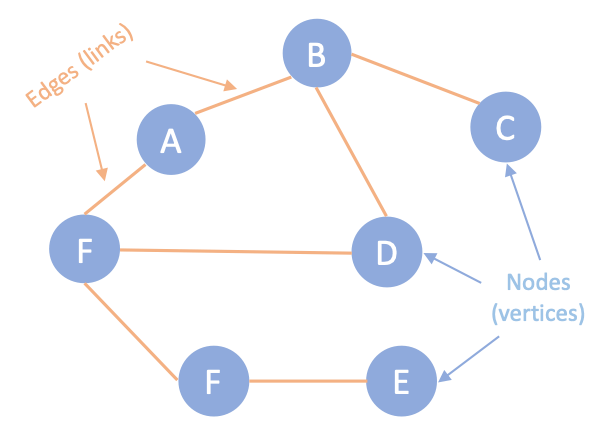
\includegraphics[width=0.5\textwidth,height=0.5\textheight,keepaspectratio]{Sections/Lit_review/Resources/basic_graphs.png}
    \caption{Basic graphs.}
    \label{fig:lit:basic_net}
\end{figure}
\FloatBarrier

% Need to address the network pathways 
Using the graph theory there has been a lot of work on analysing the pathways which is covered in \ref{}. However, the information about pathways is generally incomplete, in continuous research and a complete representation of a tissue is simply not available for most of the tissues. Therefore, there are other alternatives to analyse the gene interactions in a tissue.

% Why are we choosing the co-expressed networks?
One such approach are the co-expressed networks which uses different correlation metrics (e.g. Spearman, Pearson or partial-correlation) from gene expression to model the strengths between the nodes (edges). The rationale behind of it is that genes expressed together have a higher correlation and may represent the activation of pathways. Conversely, genes with a low correlation may be a high and low expressed genes, depicting an unrelated functioning. This approaches are covered in Section \ref{s:lit:co_net} and it is the approach used in this project as it offers a more convenient and adaptable method to other diseases or other data (multiple sources of gene expression).

\import{Sections/Lit_review/}{co-expressed_net.tex}

\import{Sections/Lit_review/}{comm_detection.tex}


\subsection{From gene to samples}

% PGCNA 

% The other paper with DEA
